\documentclass[11pt]{beamer}
\usetheme{Madrid} %тему можете свою,но нумерация слайдов обязательна
\usepackage[utf8]{inputenc}
\usepackage[OT1]{fontenc}
\usepackage[russian]{babel}
\usepackage{amsmath}
\usepackage{amsfonts}
\usepackage{amssymb}
\usepackage{alltt}
\usepackage{verbatim}
\usepackage{xcolor}
\usepackage{minted}
\usepackage{tikz} % пакет большой, разной графики и схем
\usetikzlibrary{arrows,backgrounds,positioning,fit} % дабовко к тикзету
\usemintedstyle{xcode}
\usepackage{color}
\usepackage{array, multirow} % для таблиц
\title{"Введение в компьютерную науку."}

\institute{НИЯУ МИФИ}

\subtitle{Презентация на тему:\\ "Обзор современных ЯП: Rust и Go"}
\author[Джиоев, Сметанин] % (optional)
{Т.~М.~Сметанин (teamleader) \and Н.~Д.~Джиоев\and Руководитель:~И.Ф.~Травов}



\date[2023 год] % (optional)
%------------------------------------------------------------
%The next block of commands puts the table of contents at the 
%beginning of each section and highlights the current section:

\begin{document}
%The next statement creates the title page.
\maketitle
%------------------------------------------------------------
\begin{frame}
\frametitle{Выбор компьютерной науки и работа в команде(1)}
Проект непосредственно связан с языками программирования, потому раскрывает 14 компьютерную науку: {\color{blue} (PL) Programming Languages}
Распределение задач в команде проекта было построено на основе распределения пошаговых действий:
\begin{itemize}
    \item {\color{blue}Сметанин Т.М.} - \underline{тимлид}: подготовка плана реализации проекта(1) и распределение задач по категориям(2), отбор информации и проработка шаблона Rust-части проекта(3), LaTeX оформление проекта с использованием шаблонов из Powerpoint(5)
    \item {\color{blue}Джиоев Н.Д.} - отбор информации и проработка шаблона Go-части проекта(3), вёрстка и полная разработка шаблонов обеих частей проекта с использованием иных средств создания электронных презентаций (MS Powerpoint)(4), LaTeX оформление проекта с использованием шаблонов из Powerpoint(5)
\end{itemize}
\end{frame}
\begin{frame}
\frametitle{Выбор компьютерной науки и работа в команде(2)}
Все действия распределены по пронумерованным группам, пока группа не завершена переход к следующей невозможен. Также структура повествования в Rust и Go частях разная - она отражает два подхода к изучению ЯП:
\begin{itemize}
    \item больший уклон в теорию и разбор того, что находится "под капотом"
    \item упор в практическую реализацию определённых парадигм на которых работает ЯП, создание различных pet-project-ов для понимания теории на практике, постоянное чтение документации
\end{itemize}
\end{frame}
%------------------------------------------------------------
\institute{НИЯУ МИФИ}
\title{Язык программирования Rust}
\subtitle{Выполнил Сметанин Т.М.}
%------------------------------------------------------------
\maketitle
%---------------------------------------------------------
%This block of code is for the table of contents after
%the title page
%---------------------------------------------------------
%This block of code is for the table of contents after
%the title page
\begin{frame}
\frametitle{Язык программирования \textit{Rust}: история разработки}
\begin{itemize}
    \item В 2006 году Грэйдон Хор начал разработку своего собственного языка названного в честь сорта грибов. В 2009 году Mozilla начала спонсировать его разработки. 
    \item На Mozilla Summit 2010 прошла презентация языка, ещё год шло усовершенствование компилятора и в 2011 произошла его раскрутка. 
    \item В январе 2012 была выпущена официальная альфа-версия \textit{Rust} (0.1).
    \item В мае 2015 выпущена первая стабильная версия \textit{Rust} (1.0), в которой проведена ревизия интерфейсов и возможностей языка.
    \item В декабре 2022 \textit{Rust} стал третьим языком который поддерживает в разработке ядра Linux (также поддерживаются \textit{C} и \textit{язык ассемблера}).
\end{itemize}
\end{frame}
%---------------------------------------------------------
\begin{frame}
\frametitle{История популярности}
\begin{itemize}
    \item Практически сразу с выходом языка в релиз и переходом в продакшн, он стал одним из самых держащихся на плаву ЯП. 
    \item Многие разработчики отмечали понятность документации, прозрачность языка, открытость и дружелюбность \textit{Rust}-сообщества.
    \item Первыми компаниями использовавшими этот ЯП в своих проектах стали Mozilla и Dropbox, уже в конце 2015 в Firefox для Linux часть «внутренностей» была переписана на \textit{Rust}.
\end{itemize}

\includegraphics[scale=0.6]{image.png}

\includegraphics[scale=0.6]{image2.png}
\centering
\end{frame}
%---------------------------------------------------------
\begin{frame}
\frametitle{Особенности и отличия от других языков}
\textit{Rust} предлагает несколько весомых преимуществ выгодно отличающих его от других ЯП:
\begin{itemize} 
    \item \textbf{Безопасная работа с памятью –} в \textit{Rust} отсутствует сборщик мусора и применяется специальная система работы с типами. 
    \item \textbf{Понятный и единый Packet manager –} не все высокоуровневые ЯП обладают единой системой управления пакетами, в \textit{Rust} стандартизирована единая система – {\color{orange}Cargo}.
    \item \textbf{Отсутствие дремучего legacy-кода –} \textit{Rust} это «молодой язык», в котором нет проектов и репозиториев 15-20 летней давности, которые страшно сломать при изменении в сборке проекта, то есть он лишён одной из главных проблем, например, языка \textit{C++}: эта проблема – язык \textit{C}.
\end{itemize}
\end{frame}
%---------------------------------------------------------
\begin{frame}
\frametitle{Особенности: безопасная работа с памятью}
Сегодня большинство высокоуровневых ЯП предлагают сборщик мусора ({\color{green}Garbage collector}) для ограничения контроля за управлением памятью, в то время как более низкоуровневые языки предоставляют функции такие как {\color{blue}free()} в \textit{C++} , позволяющие свободно работать с динамической памятью; из \textit{Rust} {\color{green}GC} исключён на одной из стадий пересборки компилятора. Разработчики пришли к выводу о реализации защищённости памяти без {\color{green}GC}, а с помощью системы заимствованных указателей, которые называли «ссылкой».
\begin{figure}
    \centering
    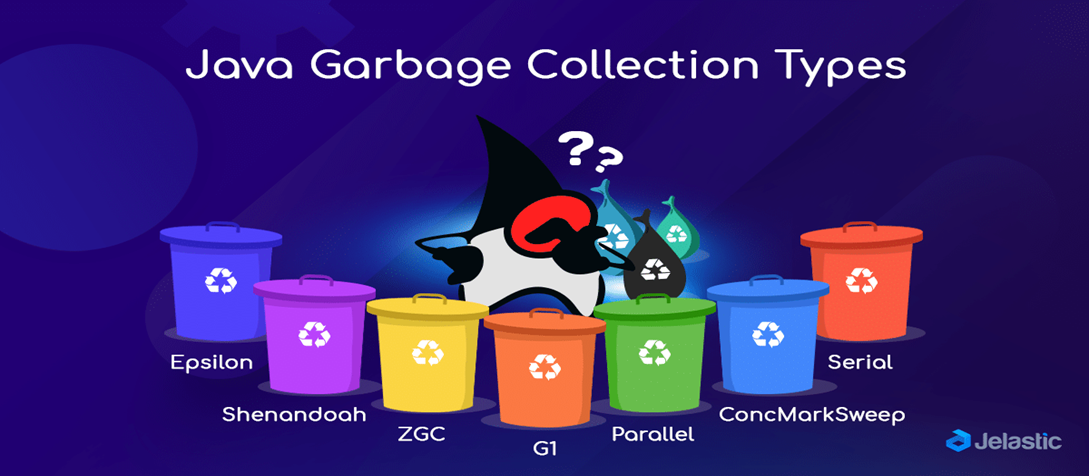
\includegraphics[width=0.7\linewidth]{image3.png}
    %\caption{}
    \label{fig:enter-label}
\end{figure}
\end{frame}
%---------------------------------------------------------
\begin{frame}
\frametitle{Особенности: безопасная работа с памятью}
В \textit{Rust} для достижения безопасности памяти применяется концепция «владения» и «заимствования»:
\begin{itemize} 
    \item По умолчанию каждая переменная является неизменяемой. 
    \item Каждое значение присваивается переменной называемой «владельцем» (“owner”). При выходе из области видимости – память освобождается.
    \item Для передачи переменной в другую часть программы используется «заимствование» - получение доступа к ссылке в памяти, без захвата самой памяти.
\end{itemize}
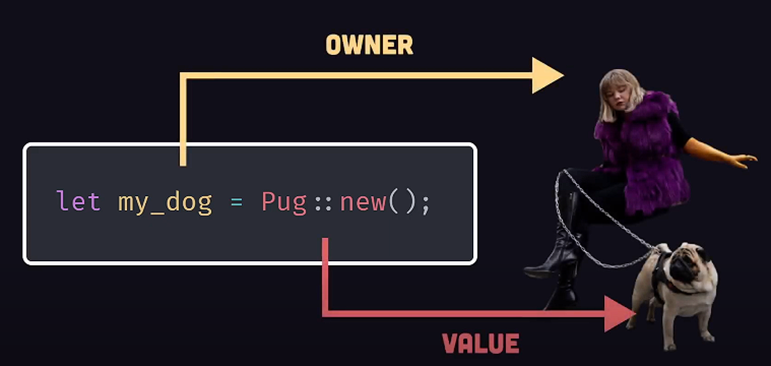
\includegraphics[width=0.4\linewidth,height=0.21\linewidth]{image4.png}
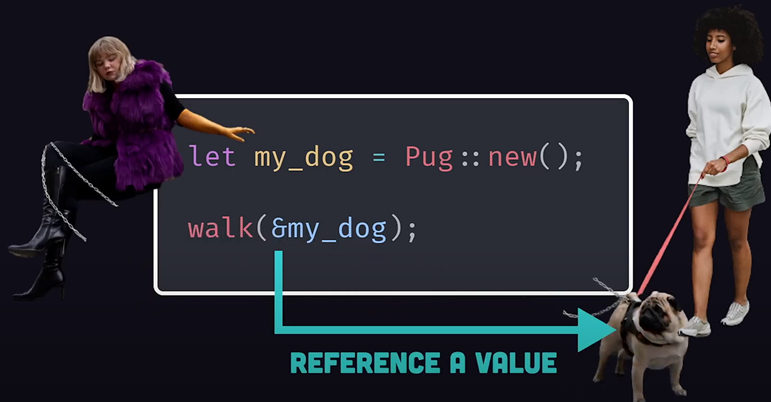
\includegraphics[width=0.4\linewidth]{image5.png}
\centering
\end{frame}
%---------------------------------------------------------
\begin{frame}[fragile]
\frametitle{Особенности: безопасная работа с памятью}
Приведём примеры работы с памятью и стандартной программы «Hello world!»:
\begin{columns} % начало 2-х колоночного режима
\column{0.4\textwidth}
\begin{minted}{rust}
let hello = "hi mom"; 
let mut hello = "hi mom";
{
let my_dog = Pug::new();
//do smthng
drop(my_dog)
}
\end{minted}
\centering
\column{0.4\textwidth}
\begin{minted}{rust}
fn main() {
log “hello, world”;
}
\end{minted}
------------------------------
\begin{minted}{rust}
fn main() {
println!(“Hello, world!”);
}
\end{minted}
\centering
\end{columns}
\end{frame}
%---------------------------------------------------------
\begin{frame}
\frametitle{Особенности: {\color{orange}packet manager - cargo}}
В современных ЯП принято использовать так называемый {\color{orange}packet manager} – систему призванную навести порядок в установленных библиотеках, открытых проектах и многом другом. Преимуществами такого подхода являются:
\begin{itemize} 
    \item Простая и понятная установка любых пакетов дополняющих ЯП 
    \item Распутывание всех зависимостей требуемых определёнными пакетами
    \item Безопасное и полное удаление пакетов и зависимостей
    \item Вменяемая работа с различными репозиториями
    \item Оптимизация и структуризация файлов исходного кода в языка с различными системами сборки
\end{itemize}
В \textit{Rust} существует единый {\color{orange}packet manager} и единая система сборки, это позволяет исключить проблему связанную с разработкой в различных {\color{blue}IDE} и различных операционных системах
\end{frame}
%---------------------------------------------------------
\begin{frame}[fragile]
\frametitle{Особенности: {\color{orange}packet manager - cargo}}
В \textit{Rust} {\color{orange}packet manager-ом} является система {\color{orange}cargo}. Её использование является более предпочтительным чем использование одного компилятора \textit{rustc}. Рассмотрим создание проекта с помощью этой системы:
\begin{minted}{console}
~#cd ~/work //перейдём в заранее выбранный каталог на ЖД
~#cargo new hello //после выполнения этой команды будет создан 
каталог hello содержащий файлы проекта
~#cd hello //по умолчанию в каталоге будет находится скрытая
папка .git, папка src с исполняемым файлом main.rs, файл 
.gitignore, файл Cargo.toml являющийся конфигурацией
проекта Cargo
~#cargo build // команда создаст исполняемый файл приложения
в папке target/debug
~#cargo run // команда построит проект и сразу запустит 
созданный файл
\end{minted}
\end{frame}
%---------------------------------------------------------
\begin{frame}
\frametitle{Особенности: {\color{orange}packet manager - cargo}}
\begin{figure}
    \centering
    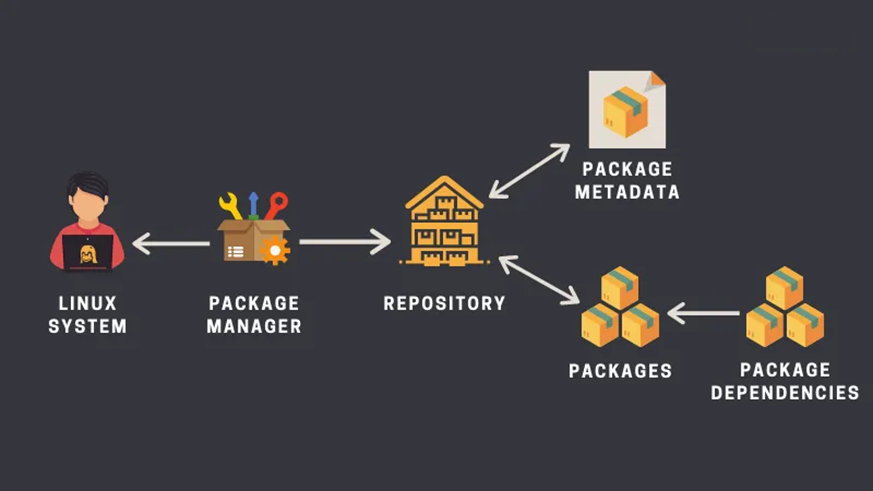
\includegraphics[width=0.7\linewidth]{image6.png}
    \caption{Принцип работы менеджера пакетов на основе linux}
\end{figure}
\centering
\end{frame}
%---------------------------------------------------------
\begin{frame}
\frametitle{Особенности: отсутствие legacy-кода}
Легаси — это код, про который говорят: «Это ещё Михалыч писал 8 лет назад для синхронизации с сервером, он работает, мы его не трогаем, потому что иначе всё сломается». При этом Михалыча в компании давно нет, документации тоже нет, и проще этот код не трогать совсем.
\begin{figure}
    \centering
    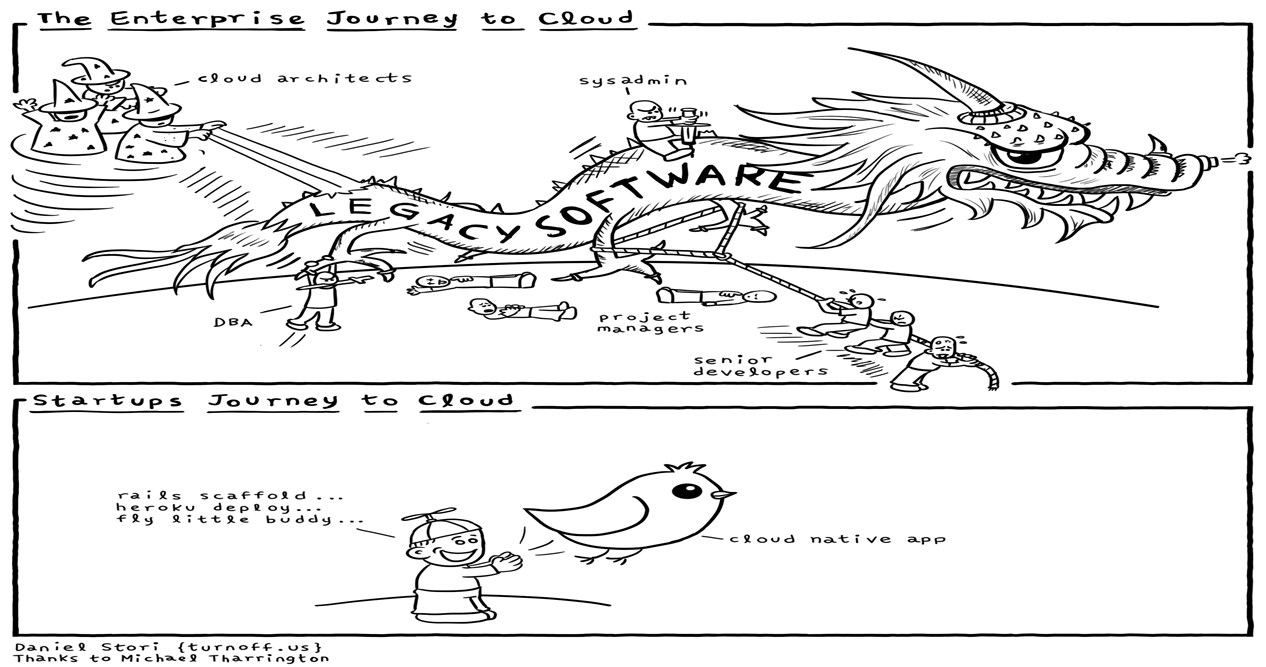
\includegraphics[width=0.85\linewidth]{image8.png}
\end{figure}
\end{frame}
%---------------------------------------------------------
\begin{frame}
\frametitle{Особенности: отсутствие legacy-кода}
\begin{figure}
    \centering
    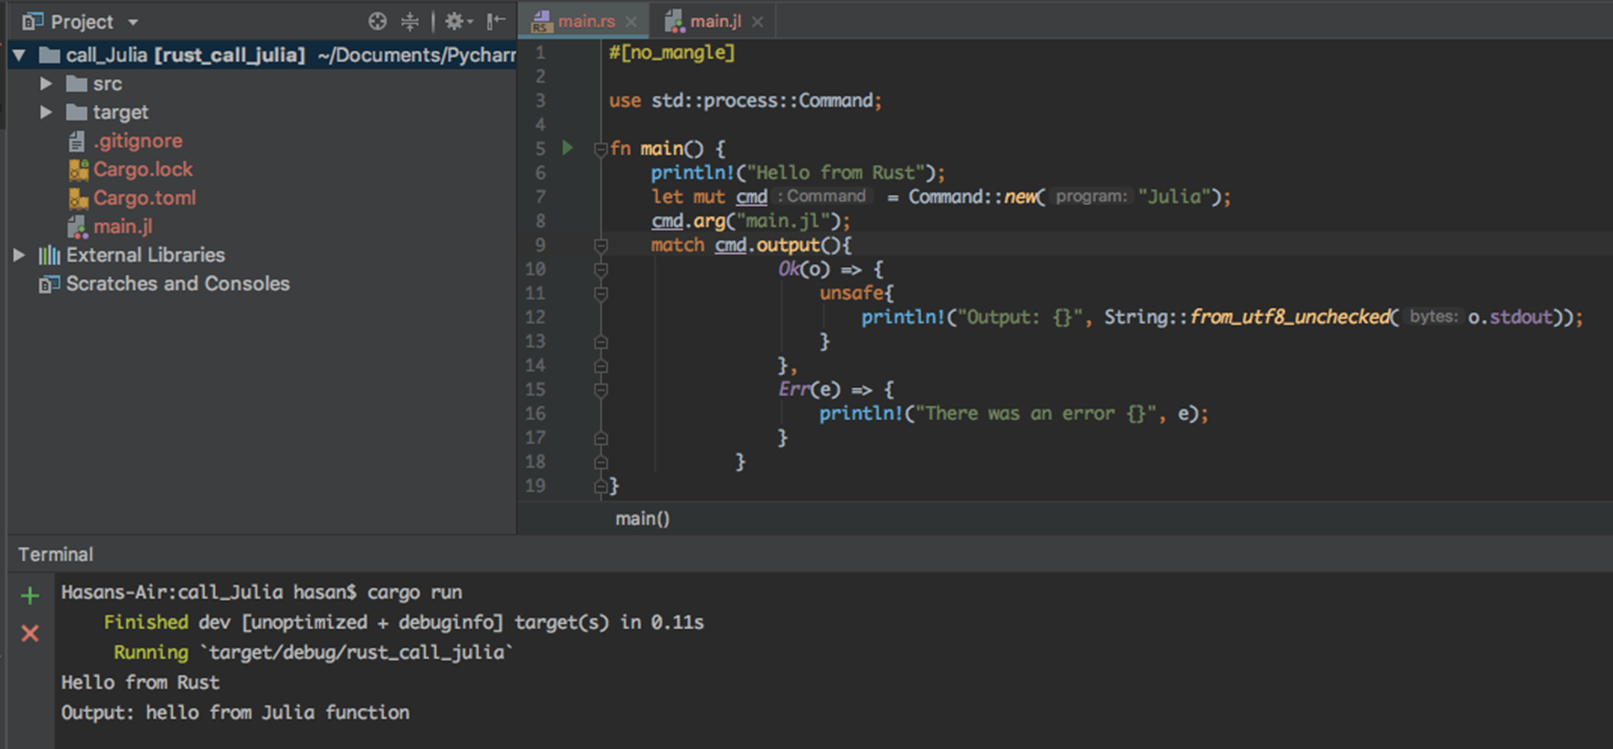
\includegraphics[width=0.85\linewidth]{image9.png}
    \caption{Скриншот из статьи датируемой 2016 годом, понятно, что код делает совсем простые вещи, но за это время он не потерял свою читаемость и понятность в современной версии языка.}
\end{figure}
\end{frame}
%---------------------------------------------------------
\begin{frame}
\frametitle{Особенности: препроцессор заменён макросами}
\begin{columns} % начало 2-х колоночного режима
\column{0.4\textwidth}
\begin{figure}
    \centering
    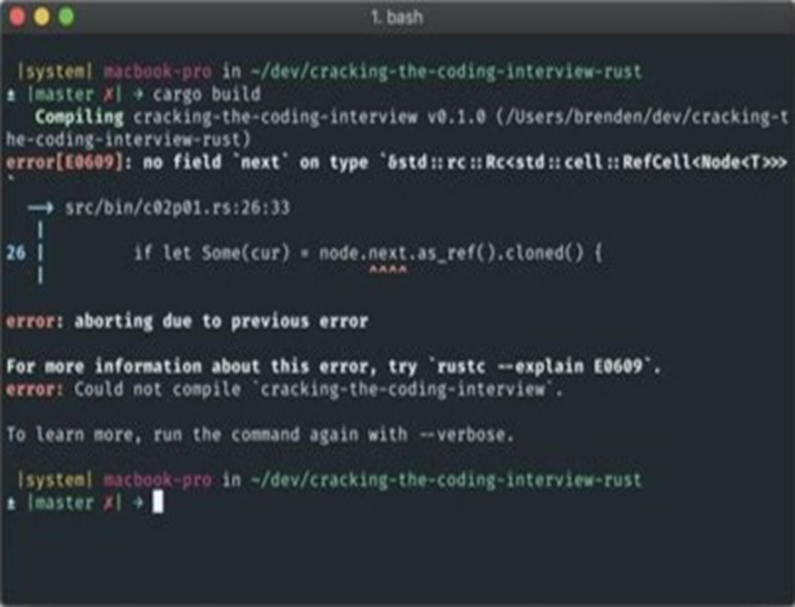
\includegraphics[width=1.2\linewidth]{image10.png}
    \caption{Читаемость ошибок и быстрое предоставление справки по ним в \textit{Rust}}
\end{figure}
\centering
\column{0.4\textwidth}
\begin{figure}
    \centering
    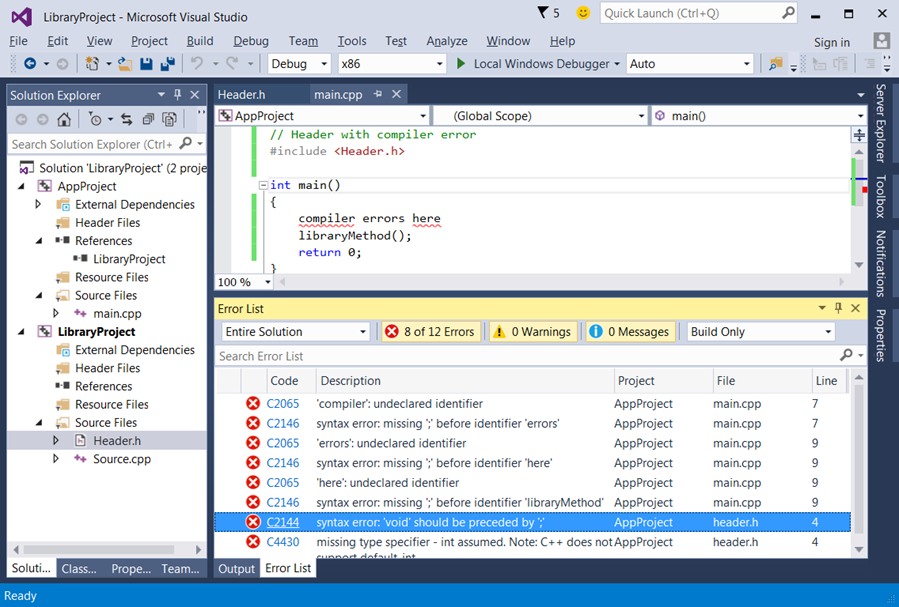
\includegraphics[width=1.2\linewidth,height=1.1\linewidth]{image11.png}
    \caption{\textit{C++}, ну тут всё понятно}
\end{figure}
\centering
\end{columns}
\end{frame}
%---------------------------------------------------------
\begin{frame}
\frametitle{Обзор по недостаткам}
Как и многие программные продукты построенные на нескольких основных парадигмах ЯП \textit{Rust} имеет ряд недостатков присущих использованию этих конкретных парадигм. Так, можно выделить следующие недостатки:
\begin{itemize} 
    \item Не ко всему программированию можно приложить системный подход, являющийся одной из главных директив \textit{Rust}.
    \item В языке большое количество сложных конструкций, требуется хорошее знание теоретических основ ЯП, сложно начать изучать \textit{Rust} как первый язык.
    \item ЯП сравнительно молод и быстро развивается, требуется постоянная слежка за трендами и обучение совершенно новым, не всегда оптимизированным вещам.
\end{itemize}
\end{frame}
%---------------------------------------------------------
\begin{frame}
\frametitle{Недостатки: системное программирование}
Rust предоставляет прекрасный контроль за использованием памяти, высокий уровень безопасности, высокую скорость исполнения и компиляции файла; это выгодно для масштабных, долгих в разработке, приспособленных под большую команду проектах, но для возможности использования такого языка от программиста требуются высокий уровень знаний и концентрации.
\begin{figure}
    \centering
    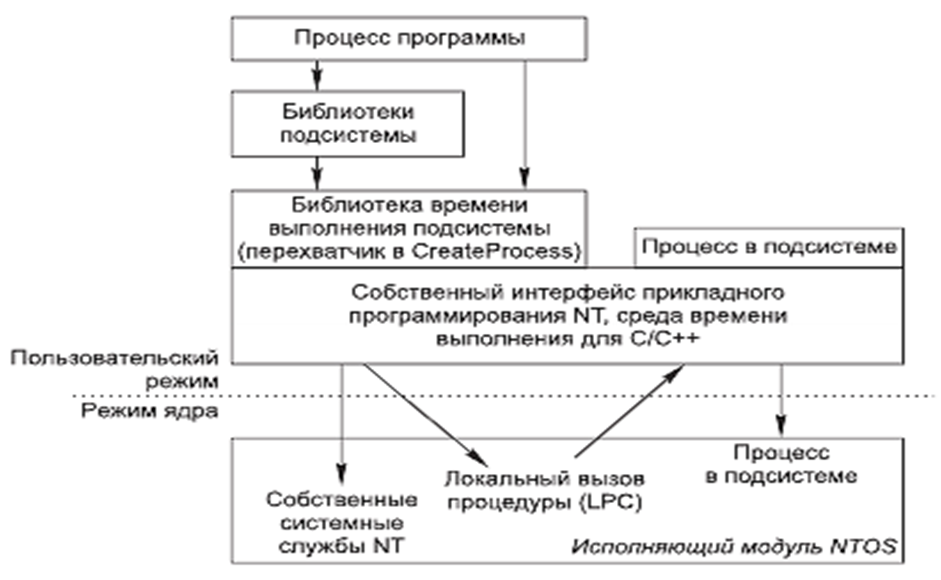
\includegraphics[width=0.5\linewidth]{image12.png}
    \caption{Обзорная схема системного подхода к программированию}
\end{figure}
\end{frame}
%---------------------------------------------------------
\begin{frame}
\frametitle{Недостатки: высокий порог вхождения}
Вместе с преимуществом, высокая безопасность и глубокий контроль памяти в Rust, это также является и его недостатком: новичок вряд ли будет использовать эти достоинства и извлекать пользу из их применения, тогда ему будет сложно разобраться в тонкостях их применения и механизме работы. Получается сам подход к созданию языка и его работе требует от программиста на нём некоторых знаний о ЯП в целом и опыта работы на других языках.
\begin{figure}
    \centering
    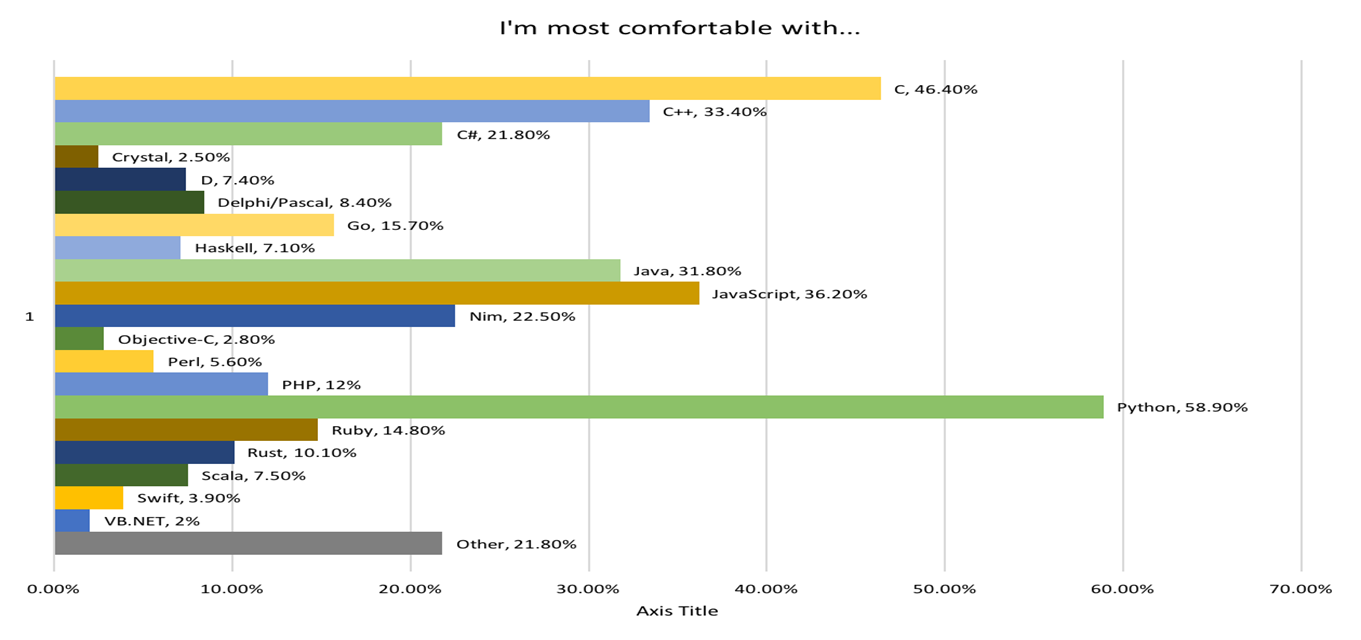
\includegraphics[width=0.8\linewidth]{image13.png}
\end{figure}
\end{frame}
%---------------------------------------------------------
\begin{frame}
\frametitle{Недостатки: молодость и незрелость языка}
Язык активно улучшается и дорабатывается, в нём реализуются многие значимые и полезные функции, но он ещё не успел накопить большой базы документации, примеров, задач, готовых enterprise проектов для обучения новичков и становления сообщества языка, как у \textit{python}, \textit{java} или \textit{C++}
\begin{figure}
    \centering
    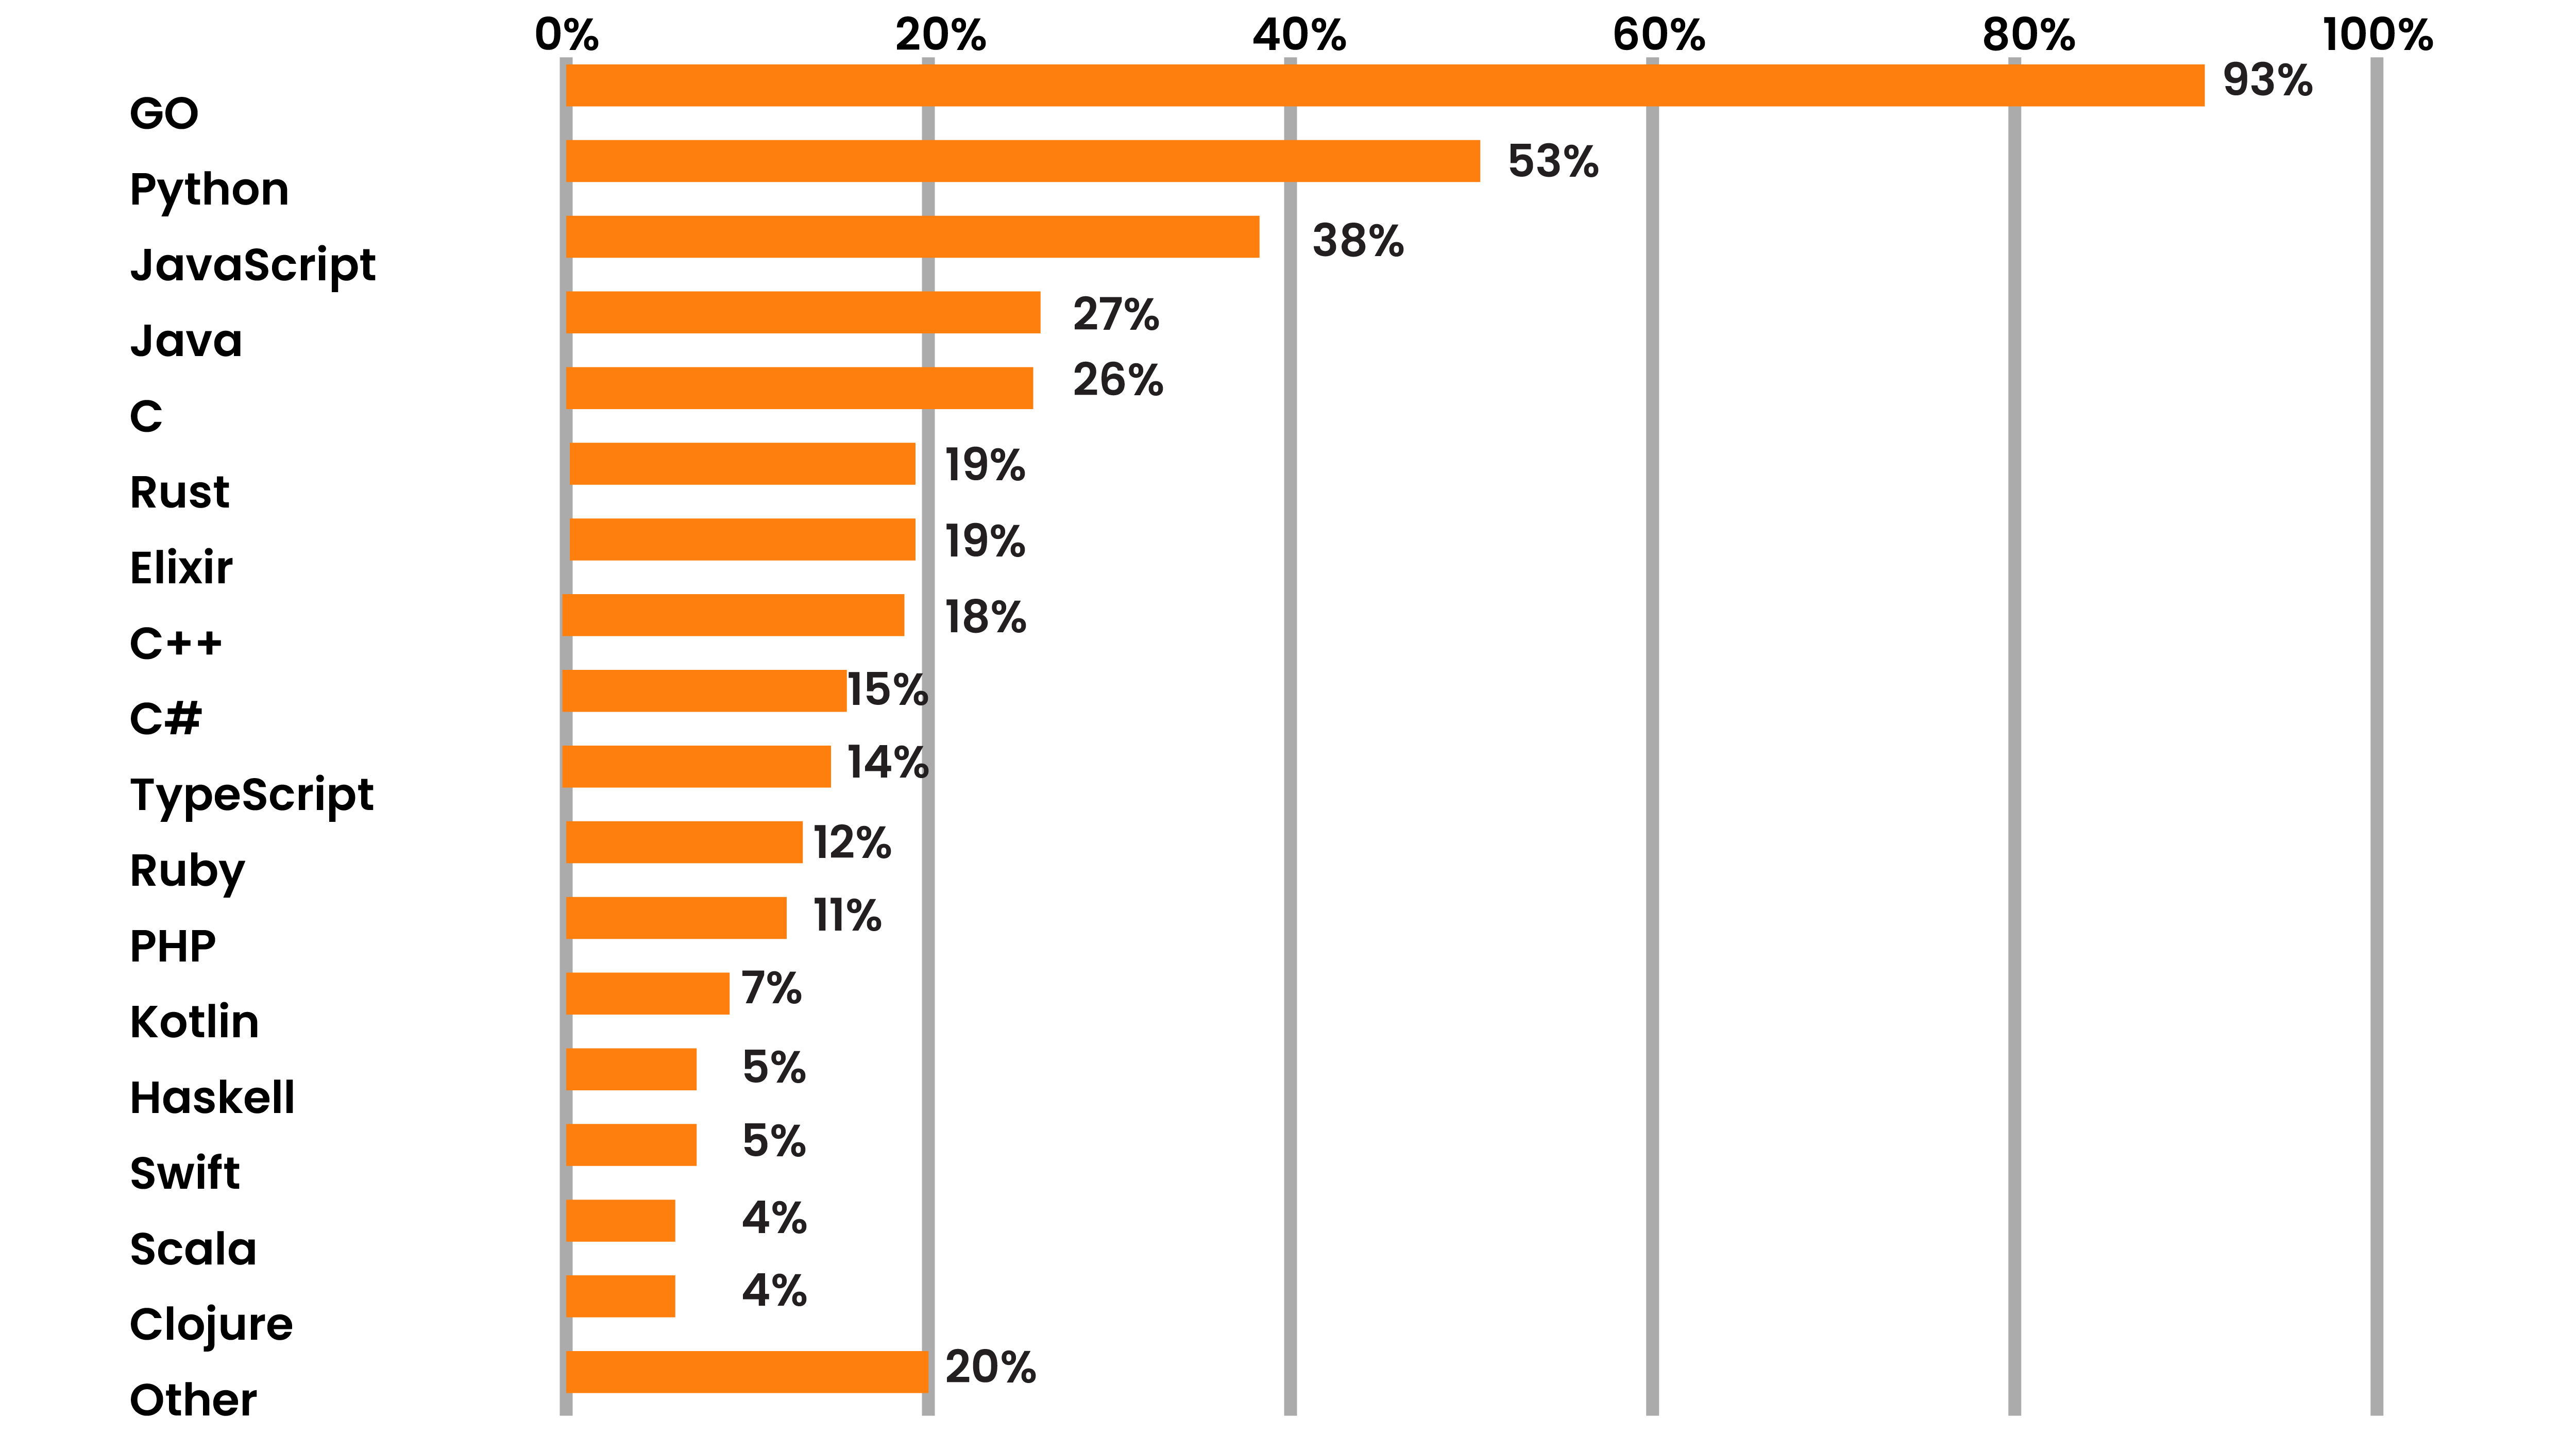
\includegraphics[width=0.8\linewidth]{image14.png}
\end{figure}
\end{frame}
%---------------------------------------------------------
\begin{frame}
\frametitle{Перспективы: вывод по особенностям}
Резюмируя, ЯП \textit{Rust} представляет собой бурно развивающийся компилируемый язык "нового поколения" значительно перерабатывающий концепцию back-end языка и языка системного программирования. За сравнительно недолгое время развития в нём реализованы:
\begin{itemize} 
    \item Действительно безопасная работа с памятью (привет \textit{C++})
    \item Хорошая единая система сборки совмещённая с {\color{orange}packet manager-ом}
    \item Замена препроцессору в виде макросов, что позволяет обеспечить читаемость ошибок компиляции
\end{itemize}
\end{frame}
%---------------------------------------------------------
\begin{frame}
\frametitle{Перспективы: вывод по недостаткам}
В силу своих особенностей (являющихся в общем-то преимуществами) \textit{Rust} имеет ряд недостатков, которые могут отпугнуть начинающих программистов или программистов с задачами требующими минимальных временных затрат (например большое количство стартапов сейчас реализуется на \textit{Go} так как он позволяет меньше внимания уделять работе с памятью и низкоуровневым моментам в целом).
\begin{figure}
    \centering
    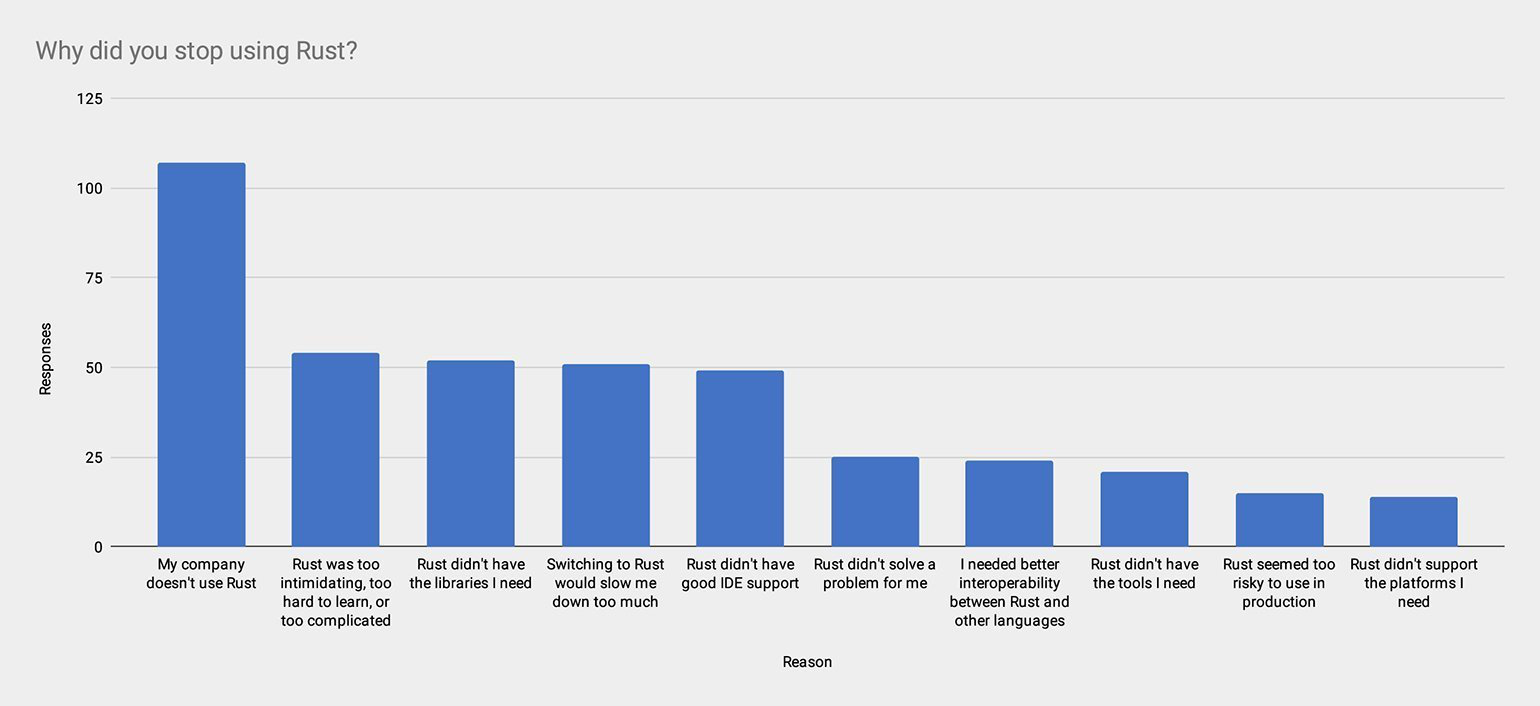
\includegraphics[width=0.9\linewidth]{image15.png}
\end{figure}
\end{frame}
%---------------------------------------------------------
\begin{frame}
\frametitle{Бонус - участники конференции RustCon2021 в Москве отвечают на вопрос: "За что я люблю \textit{Rust?}"}
\begin{itemize} 
    \item "В \textit{Rust}-е? Typesafety относительно плюсов (\textit{C++})"
    \item "Скорость и отсутствие runtime-a"
    \item "Для меня самое главное - это возможность адекватно работать с ошибками"
    \item "Для меня в \textit{Rust}-е самое главное, что он сделан для людей, а не для машины"
    \item "Безопасность, безопасная разработка"
\end{itemize}
\end{frame}
%---------------------------------------------------------
%---------------------------------------------------------
%---------------------------------------------------------
\title{Язык программирования Go}
\subtitle{Выполнил Джиоев Н.Д.}
%---------------------------------------------------------
\frame{\titlepage}
%---------------------------------------------------------
\begin{frame}
\frametitle{Язык программирования \textit{Go}: История создания}
\textit{Go} (часто также \textit{golang}) — компилируемый многопоточный язык программирования, разработанный внутри компании Google. Разработка \textit{Go} началась в сентябре 2007 года, его непосредственным проектированием занимались Роберт Гризмер, Роб Пайк и Кен Томпсон, занимавшиеся до этого проектом разработки операционной системы Inferno. Официально язык был представлен в ноябре 2009 года.
\begin{figure}
    \centering
    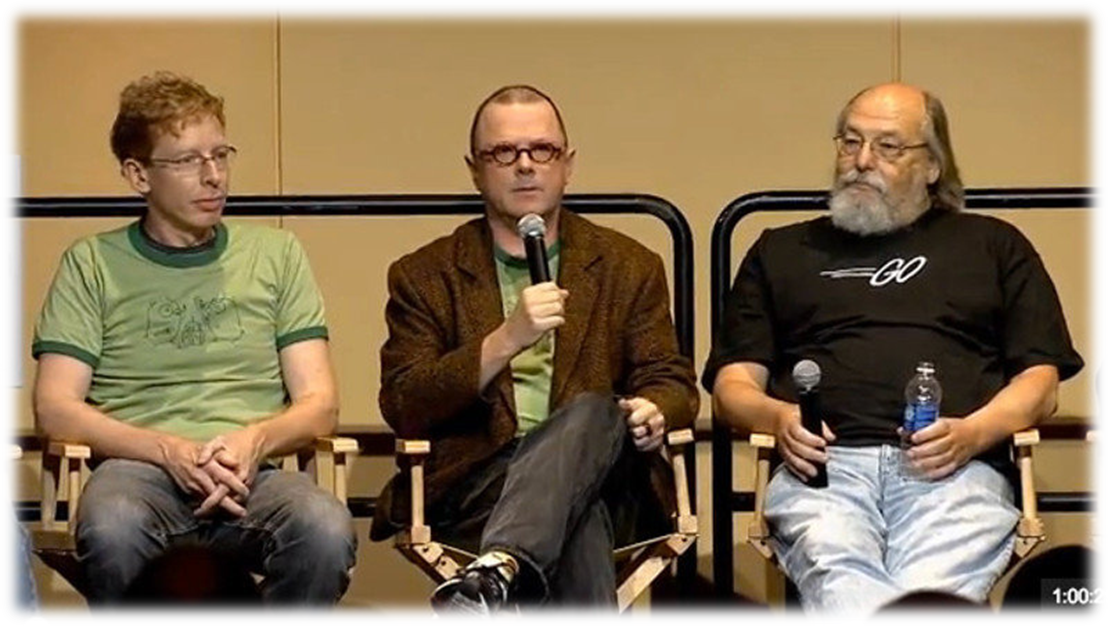
\includegraphics[width=0.6\linewidth]{image16.png}
\end{figure}
\end{frame}
%---------------------------------------------------------
\begin{frame}
\frametitle{Назначение языка \textit{Go} и его идеология}
Язык \textit{Go} разрабатывался как язык программирования для создания высокоэффективных программ, работающих на современных распределённых системах и многоядерных процессорах. Он может рассматриваться как попытка создать замену языкам \textit{С} и \textit{C++} с учётом изменившихся компьютерных технологий и накопленного опыта разработки крупных систем. 
\begin{figure}
    \centering
    
\includegraphics[width=0.7\linewidth]{image17.png}
\end{figure}
\end{frame}
%---------------------------------------------------------
\begin{frame}
\frametitle{Назначение языка \textit{Go} и его идеология}
По словам Роба Пайка «\textit{Go} был разработан для решения реальных проблем, возникающих при разработке программного обеспечения в Google». В качестве основных таких проблем он называет:
\begin{itemize} 
    \item Медленную сборку программ
    \item Неконтролируемые зависимости
    \item Использование разными программистами разных подмножеств языка
    \item Затруднения с пониманием программ, вызванные неудобочитаемостью кода, плохим документированием и так далее
    \item Дублирование разработок
    \item Высокую стоимость обновлений
    \item Несинхронные обновления при дублировании кода
    \item Сложность разработки инструментария
\end{itemize}
\end{frame}
%---------------------------------------------------------
\begin{frame}
\frametitle{Назначение языка \textit{Go} и его идеология}
Основными требованиями к языку стали:
\begin{itemize} 
    \item Ортогональность - язык должен предоставлять небольшое число средств, не повторяющих функциональность друг друга
    \item Простая и легкоразбираемая грамматика с минимумом ключевых слов
    \item Простая работа с типами - типизация должна обеспечивать безопасность, но не превращаться в бюрократию, лишь увеличивающую код
    \item Отказ от иерархии типов, но с сохранением объектно-ориентированных возможностей
    \item Отсутствие неявных преобразований
    \item {\color{green}Сборка мусора}
\end{itemize}
\end{frame}
%---------------------------------------------------------
\begin{frame}
\frametitle{Основные возможности языка}
\begin{itemize} 
    \item \textit{Go} — язык со строгой статической типизацией. Доступен автоматический вывод типов, для пользовательских типов — «утиная типизация»
    \item Полноценная поддержка указателей, но без возможности применять к ним арифметические операции
    \item Строковый тип со встроенной поддержкой юникода
    \item Использование динамических массивов (срезов),хеш-таблиц (словарей), вариант цикла для обхода коллекции
    \item Средства функционального программирования
    \item Автоматическое управление памятью со сборщиком мусора
    \item Средства объектно-ориентированного программирования ограничиваются интерфейсами
    \item Средства параллельного программирования
\end{itemize}
\end{frame}
%---------------------------------------------------------
\begin{frame}
\frametitle{Алфавит}
\textit{Go} — регистрозависимый язык с полной поддержкой Юникода в строках и идентификаторах.
Идентификатор традиционно может быть любой непустой последовательностью, включающей буквы, цифры и знак подчёркивания, начинающийся с буквы и не совпадающий ни с одним из ключевых слов языка \textit{Go}. При этом под «буквами» понимаются все символы Юникода, относящиеся к категориям «Lu», «Ll», «Lt», «Lm» или «Lo», под «цифрами» — все символы из категории «Nd». Все ключевые слова \textit{Go} пишутся в нижнем регистре. Переменные, начинающиеся с заглавных букв, являются экспортируемыми (public), а начинающиеся со строчных букв — неэкспортируемыми (private).
\end{frame}
%---------------------------------------------------------
\begin{frame}[fragile]
\frametitle{Работа с пакетами}
Любая программа на \textit{Go} включает один или несколько пакетов. Пакет, к которому относится файл исходного кода, задаётся описанием package в начале файла. Система пакетов \textit{go}-среды имеет древовидную структуру, аналогичную дереву каталогов. Для использования в файле кода Go объектов, экспортированных другим пакетом, пакет должен быть импортирован, для чего применяется конструкция import.
\begin{minted}{golang}
package main
/* Импорт */
import (
    "fmt"           // Стандартный пакет для вывода
    "database/sql"  // Импорт вложенного пакета
    w "os"          // Импорт с псевдониммом
    . "math"        // Импорт без квалификации
    _ "gopkg.in/goracle.v2" // Пакет не имеет явного кода
)
\end{minted}
\end{frame}
%---------------------------------------------------------
\begin{frame}[fragile]
\frametitle{Система циклов, оператор for}
В \textit{Go} для организации всех видов циклов используется циклическая конструкция {\color{blue}for}:
\begin{minted}{golang}
for i < 10 {} // цикл с предусловием, аналог while в С
for i := 0; i < 10; i++ {} // цикл со счётчиком, как for в С
for {} // бесконечный цикл
    // Выход из цикла должен быть организован вручную,
    // используются конструкций return или break
for { // цикл с постусловием
  ... // тело цикла
  if i>=10 {break}
}
for i, v := range arr {} // цикл по коллекции arr
// i - индекс (или ключ) текущего элемента
// v - копия значения текущего элемента массива
\end{minted}
\end{frame}
%---------------------------------------------------------
\begin{frame}[fragile]
\frametitle{Оператор множественнного выбора switch}
Синтаксис оператора {\color{blue}switch} имеет ряд особенностей. Прежде всего, в отличие от \textit{C}, не требуется использование оператора {\color{blue}break}: после отработки выбранной ветви исполнение завершается. Если необходимо продолжение работы, то требуется использовать оператор {\color{blue}fallthrough}:
\begin{minted}{golang}
switch value {
case 1:
    fmt.Println("One")
    fallthrough // Далее будет выполнена ветвь "case 0:"
case 0:
    fmt.Println("Zero")
}
\end{minted}
\end{frame}
%---------------------------------------------------------
\begin{frame}
\frametitle{Особенности архитектуры: обработка ошибок}
Язык \textit{Go} не поддерживает типичного для большинства современных языков синтаксиса структурной обработки исключений. Вместо этого рекомендуется использовать возврат ошибки как одного из результатов функции:
\begin{itemize} 
    \item В последнем параметре функция возвращает объект-ошибку либо пустой указатель {\color{yellow}nil}, если функция выполнилась без ошибок.
    \item Возвращённый функцией объект проверяется и ошибка, если она возникла, обрабатывается.
    \item Проигнорировать ошибку, возвращаемую из функции.
    \item При возникновении фатальных ошибок, делающих невозможным дальнейшее исполнение программы, возникает состояние {\color{yellow}«паники» (panic)}, которое по умолчанию приводит к аварийному завершению программы с выдачей сообщения об ошибке.
\end{itemize}
\end{frame}
%---------------------------------------------------------
\begin{frame}[fragile]
\frametitle{Особенности архитектуры: обработка ошибок}
\begin{minted}{golang}
func ReadFile(srcName string)(result string, err error) {
    file, err := os.Open(srcName)
    if err != nil {
    // Генерация новой ошибки с уточняющим текстом
    return nil, fmt.Errorf("чтение файла %q: %w", srcName, err)
    }
    ...// Дальнейшее исполнение функции, если ошибки не было
    return result, nil // Возврат результата и пустой ошибки
}
\end{minted}
\end{frame}
%---------------------------------------------------------
\begin{frame}[fragile]
\frametitle{Особенности архитектуры: обработка ошибок}
\begin{minted}{golang}
func main() {
	defer func() {
		err := recover()
		if v, ok := err.(error); ok {
			fmt.Fprintf(os.Stderr, 
            "Error %v \"%s\"\n", err))
		} else if err != nil {panic(err)}
	}()
	a, err := strconv.ParseInt(os.Args[1], 10, 64)
	if err != nil {panic(err)}
	b, err := strconv.ParseInt(os.Args[2], 10, 64)
	if err != nil {panic(err)}
	fmt.Fprintf(os.Stdout, "%d / %d = %d\n", a, b, a/b)
}
\end{minted}
\end{frame}
%---------------------------------------------------------
\begin{frame}
\frametitle{Особенности архитектуры: обработка ошибок}
В примере выше могут произойти ошибки при преобразовании аргументов программы в целые числа функцией {\color{purple}strconv.ParseInt()}. Также возможна паника при обращении к массиву {\color{brown}os.Args} при недостаточном количестве аргументов, либо при делении на нуль, если второй параметр окажется нулевым. При любой ошибочной ситуации генерируется паника, которая обрабатывается в вызове {\color{purple}defer}.
\end{frame}
%---------------------------------------------------------
\begin{frame}
\frametitle{Особенности архитектуры: низкоуровневое программирование}
Средства низкоуровневого доступа к памяти сосредоточены в системном пакете {\color{yellow}unsafe}.{\color{yellow}Unsafe} предоставляет функции:
\begin{itemize} 
    \item {\color{blue}unsafe.Sizeof()} — аргументом может быть выражение любого типа, функция возвращает реальный размер операнда в байтах, включая неиспользуемую память, которая может появляться в структурах из-за выравнивания
    \item {\color{blue}unsafe.Alignof()} — аргументом может быть выражение любого типа, функция возвращает размер в байтах, по которому типы операнда выравниваются в памяти
    \item {\color{blue}unsafe.Offsetof()} — аргументом должно быть поле структуры, функция возвращает смещение в байтах, по которому располагается это поле в структуре
    \item пакет предоставляет тип {\color{brown}unsafe.Pointer}, в который может быть преобразован любой указатель и указатель любого типа
\end{itemize}
\end{frame}
%---------------------------------------------------------
\begin{frame}
\frametitle{Особенности архитектуры: низкоуровневое программирование}
Описанные преобразования могут быть небезопасны, поэтому их рекомендуют по возможности избегать:
\begin{itemize}
    \item Во-первых, возможны очевидные проблемы, связанные с ошибочным обращением не к той области памяти
    \item Более тонким моментом является то, что несмотря на использование пакета {\color{yellow}unsafe}, объекты \textit{Go} продолжают находиться под управлением менеджера памяти и {\color{green}сборщика мусора}
    \item Поскольку спецификация \textit{Go} не даёт точных указаний на то, в какой мере программист может рассчитывать на сохранение актуальности преобразованного в число указателя, существует рекомендация: \textbf{сводить подобные преобразования к минимуму}
\end{itemize}
\end{frame}
%---------------------------------------------------------
\begin{frame}
\frametitle{Реализации}
На данный момент существуют два основных компилятора \textit{Go}:
\begin{itemize}
    \item \textbf{gc} — общее название для официального набора инструментов разработки, поддерживаемого группой разработчиков языка. Первоначально он включал компиляторы для {\color{brown}amd64}, для {\color{brown}x86}, для {\color{brown}ARM} и был написан на \textit{С}. В версии 1.5 весь код на \textit{С} был переписан на \textit{Go} и \textit{языке ассемблера}
    \item \textbf{gccgo} — компилятор \textit{Go} с клиентской частью, написанной на \textit{C++}, и рекурсивным парсером.
\end{itemize}
Также существуют проекты:
\begin{itemize}
    \item \textbf{llgo} — прослойка для компиляции \textit{Go} в llvm, написанная на самом Go 
    \item \textbf{gollvm} — проект компиляции \textit{Go} через систему компиляторов LLVM, развиваемый Google
    \item \textbf{SSA interpreter} — интерпретатор, позволяющий запускать программы на \textit{Go}
\end{itemize}
\end{frame}
%---------------------------------------------------------
\begin{frame}
\frametitle{Средства разработки}
Среда разработки \textit{Go} содержит несколько инструментов командной строки: утилиту \textit{Go}, обеспечивающий компиляцию, тестирование и управление пакетами, и вспомогательные утилиты {\color{blue}godoc} и {\color{blue}gofmt}. На текущий момент доступны две {\color{blue}IDE}, изначально ориентированные на язык \textit{Go} — это проприетарная {\color{blue}GoLand} (разрабатывается в JetBrains на платформе {\color{blue}IntelliJ}) и свободная {\color{blue}LiteIDE} (ранее проект назывался {\color{blue}GoLangIDE}).
Также Go поддерживается плагинами в универсальных IDE {\color{blue}Eclipse}, {\color{blue}NetBeans}, {\color{blue}Komodo}, {\color{blue}Visual Studio}, {\color{blue}Zeus} и других. Автоподсветка, автодополнение кода на \textit{Go} и запуск утилит компиляции и обработки кода реализованы в виде плагинов к более чем двум десяткам распространённых текстовых редакторов под различные платформы.
\end{frame}
%---------------------------------------------------------
\begin{frame}[fragile]
\frametitle{Финиш по обзору современных ЯП}
...the End по языкам \textit{Rust} и \textit{Go}, вопросы? 
\begin{minted}{python}

вопросы = int(input())
if(вопросы == 0):
    print("Спасибо за ваше внимание!)
else:
    вопросы-=1
\end{minted}
\centering
\end{frame}
%---------------------------------------------------------
\end{document}